\documentclass[a4paper,10pt]{article}
\usepackage[utf8]{inputenc}
\usepackage{graphicx}
\usepackage[rflt]{floatflt}
\usepackage[sf, bf]{caption}

\setlength{\parindent}{1em}

\begin{document}
    \huge 
    \noindent
    \textbf{Brunn User Documentation}

    \normalsize

    \section{General Bioclipse Structure}

        \subsection{Editors and Views}
            Bioclipse is made up of editors and views. Editors are for editing
            things. Things can be opened in an editor, edited and then saved
            and the editor closed. A view can listen to what is selected. For
            example the properties view show the properties of the item
            currently selected. Figure \ref{editorsAndViews} shows what are
            views and what are editors in a standard Brunn window.
            \begin{figure}[htbp]
                \begin{center}
                    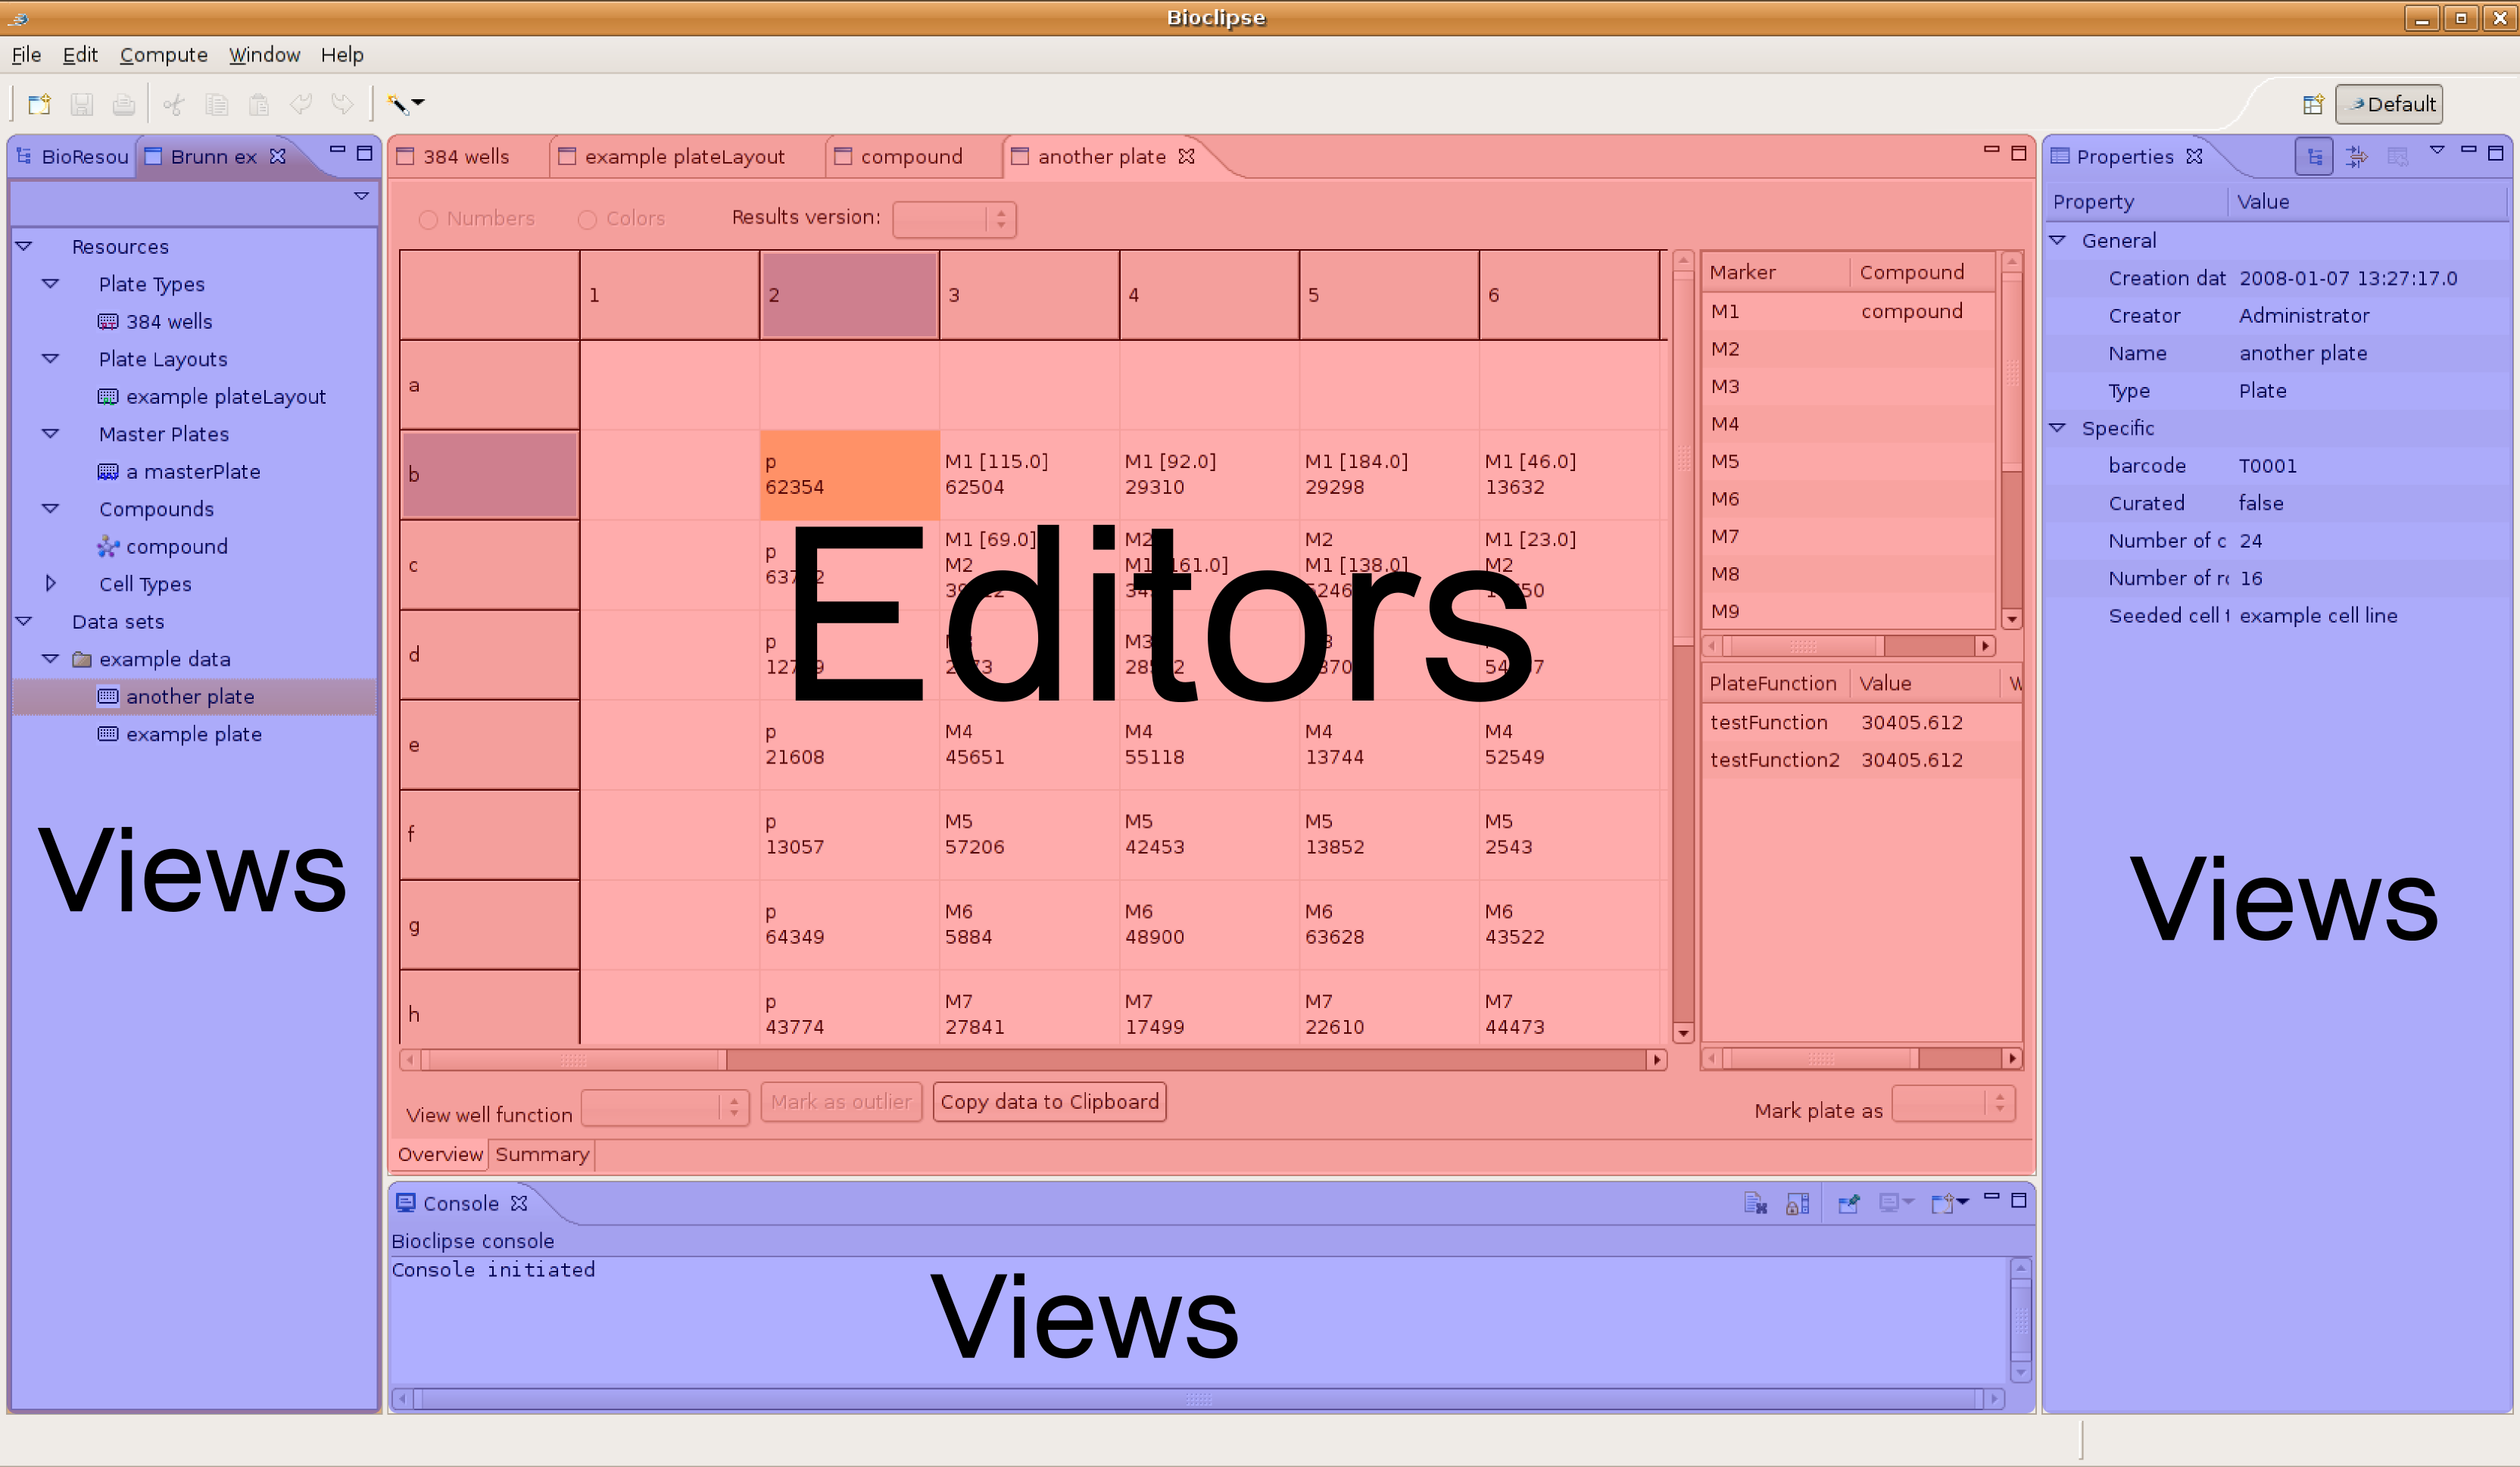
\includegraphics[width=1\textwidth]{images/EditorsViews.png}
                \end{center}
                \caption{\textit{The Bioclipse workspace consists of editors
                                 and views. The editors are stacked in the
                                 middle and the views can be moved around.}}
                \label{editorsAndViews}
            \end{figure}

        \subsection{Two ``hidden'' but important menus}

            There are two menues in the Eclipse structure that can be
            hard to find. Figure \ref{viewMenu} points them out. One contains
            operations coupled to a view and can be found (in a view that has
            it) when clicking a little triangle in the upper right corner of a
            view. The other switches between different tabs in a multipage
            editor. Not all editors have multiple pages.
            \begin{figure}[htbp]
                \begin{center}
                    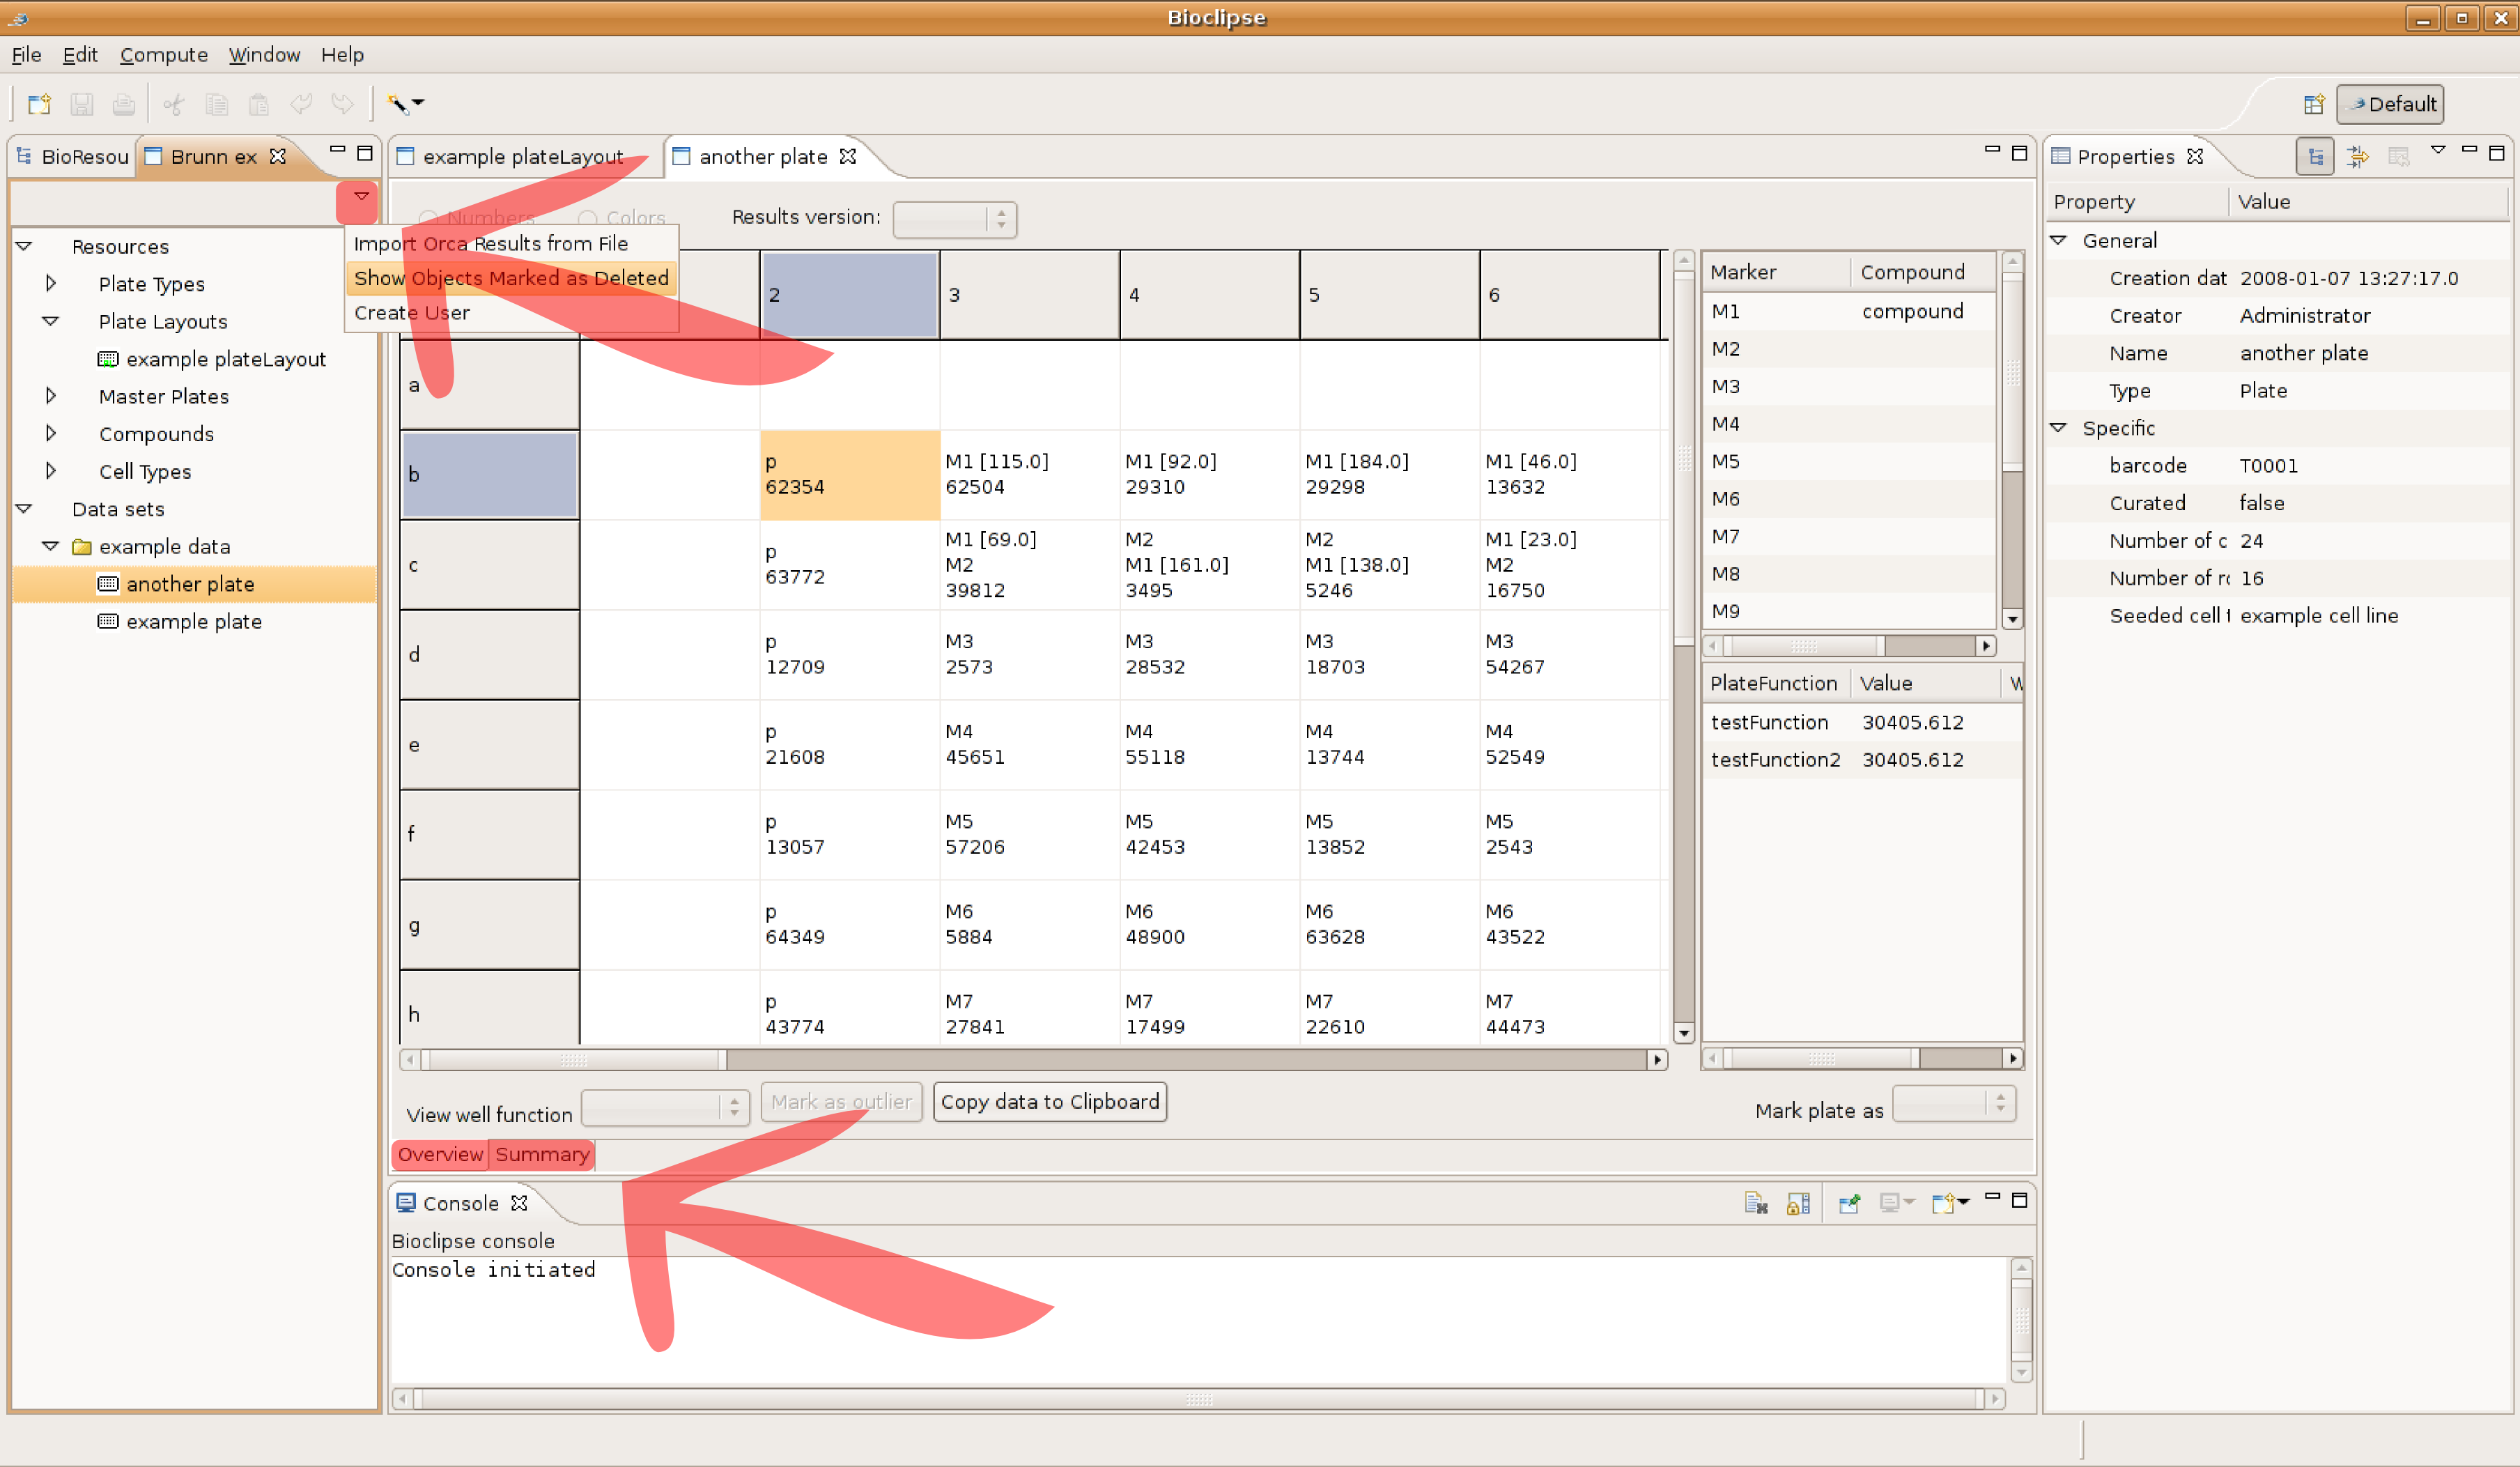
\includegraphics[width=1\textwidth]{images/twoMenues.png}
                \end{center}
                \caption{\textit{A view can have a menu. They are very
                    convenient but can be hard to spot the first time. They are
                    just little triangles in the corner of the view. Editors
                    can have multiple pages but also this feature can be hard
                    to spot. The tabs at the bottom of the editor switch
                    between pages.}}
                \label{viewMenu}
            \end{figure}

    \section{Brunn}
        
         A few general tips for the Brunn user:
         \begin{itemize}
             \item Double clicking an item opens it up for editing
             \item Right clicking often opens up a context menu with
                   operations. If you wonder about how to do somehing, try
                   right clicking.
         \end{itemize}


        \begin{figure}[htbp]
            \begin{center}
                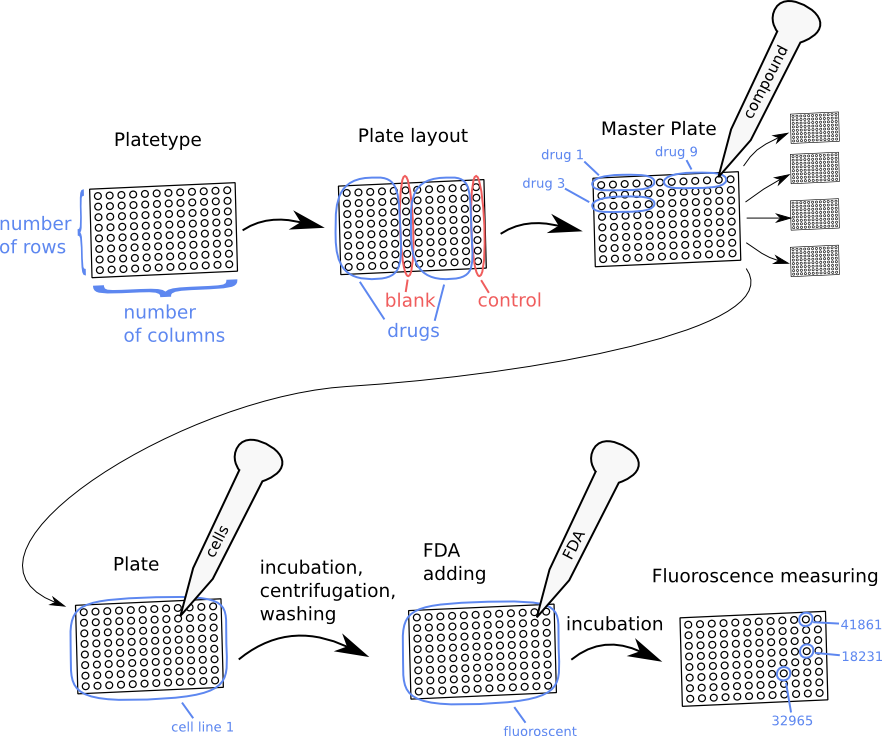
\includegraphics[width=1\textwidth]{images/labWork.png}
            \end{center}
            \caption{\textit{A description of how the items of Brunn fits into
                             the work performed in the lab. In the system a
                             plate type defines the size, number of columns and
                             rows, of a plate. A plate layout defines where on
                             the plate the controls and the compounds are to be
                             placed. Based upon this plate layout a number of
                             equal plates are made, conforming to a so-called
                             “master plate” that defines which drugs are placed
                             in which wells.}}
            \label{labWork}
        \end{figure}

         \subsection{Installation and Set-Up}
         \texttt{TODO:}Write stuff here

         \subsection{The Brunn Explorer View} 
            \begin{floatingfigure}{0.3\textwidth}
                \begin{center}
                    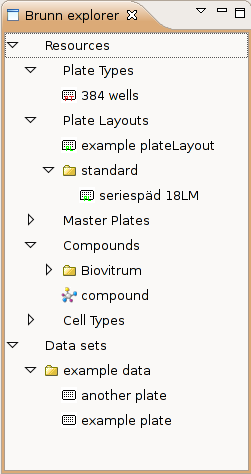
\includegraphics[width=.2\textwidth]
                                    {images/explorerView.png}
                \end{center}
                \caption{\textit{The Brunn Explorer view is used to browse the
                    system}}
                \label{explorerView}
            \end{floatingfigure}

            \noindent
            The first time Brunn is started the Brunn Explorer View might not
            be shown. It can be made visible by clicking:
            \texttt{Window$\rightarrow$Show View$\rightarrow$Other\ldots} and
            under Brunn choose Brunn Explorer. 

            Double clicking something in the explorer view opens that thing in
            an editor. The explorer view is where new things are created. The
            various items of the tree have context menus that appear when right
            clicked. For example, folders can be created and dragged and
            dropped into anod out of. Figure \ref{labWork} explains how the
            different items in the tree fits in to what is done in the lab.
            
            In Brunn almost nothing can be deleted. However, things can be
            marked as deleted, meaning that they won't show up unless the menu
            alternative \texttt{show objects marked as deleted} is choosen in
            the views menu. In this menu there also is a wizard for importing
            result data and a way to create a new user account. The
            alternatives to show objects marked as deleted and create users are
            only there if the loggged in user has administrator access.
        
        \subsection{Creating items}
            New items are created by right-clicking a folder that is either the
            the top folder for the sort of item to be created or a subfolder of
            it, and then choosing a create operation. This opens some dialog
            where things special for that sort of item can be entered. 

            So for example to create a plate layout start by right clicking the
            folder \texttt{Plate Layouts} and choose \texttt{Create Plate
            Layout}. In the dialog that shows up, choose one plate type to base
            the platelayout on, and enter a name for your new plate layout.
            Then click Ok to create the plate layout.

        \subsection{Plate Type} A plate type defines the size of a plate. It
            simply holds number of rows and number of columns of a plate. 

        \subsection{Plate Layout}
            A plate layout defines which wells on a plate should be used for
            compounds, controls or just be left empty. The plate layout is also
            where calculation functions are defined. For example, survival
            index and variation over the wells marked as positive control. 

            \subsubsection{Adding markers to a plate layout}
                \begin{figure}[htbp]
                    \begin{center}
                        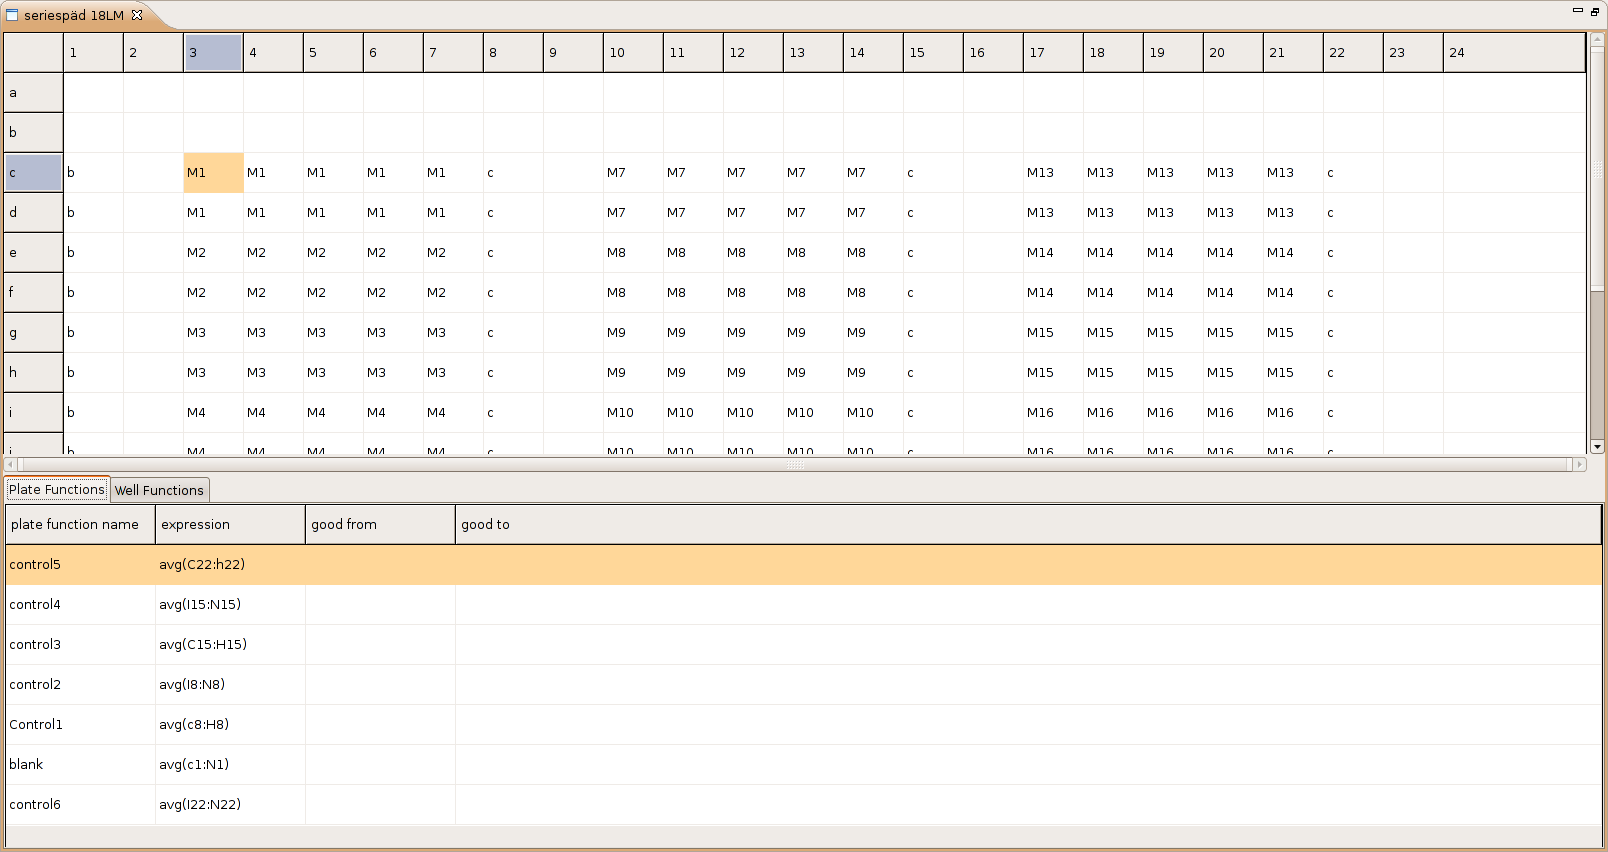
\includegraphics[width=1\textwidth]
                                        {images/plateLayoutEditor.png}
                    \end{center}
                    \caption{\textit{The platelayouteditor}}
                    \label{platelayoutEditor}
                \end{figure}
            \subsubsection{Defining calculation functions on a plate layout}

        \subsection{Master Plate}
            A master plate defines which compound marker correspond to which
            compound and with what concentration.
            
            \subsubsection{Defining compound for a compound marker}

        \subsection{Plate}
        \texttt{TODO:}Write stuff here

\end{document}

